% Created 2019-11-12 mar 16:15
\documentclass[presentation,aspectratio=169]{beamer}
\usepackage[utf8]{inputenc}
\usepackage[T1]{fontenc}
\usepackage{fixltx2e}
\usepackage{graphicx}
\usepackage{longtable}
\usepackage{float}
\usepackage{wrapfig}
\usepackage{rotating}
\usepackage[normalem]{ulem}
\usepackage{amsmath}
\usepackage{textcomp}
\usepackage{marvosym}
\usepackage{wasysym}
\usepackage{amssymb}
\usepackage{hyperref}
\tolerance=1000
\usepackage{khpreamble}
\usepackage{xcolor}
\newcommand{\sign}{\mathrm{sign}}
\renewcommand{\transp}{^{\mathrm{T}}}
\usetheme{default}
\author{Kjartan Halvorsen}
\date{2019-11-13}
\title{Robust Kalman filter}
\hypersetup{
  pdfkeywords={},
  pdfsubject={},
  pdfcreator={Emacs 25.3.50.2 (Org mode 8.2.10)}}
\begin{document}

\maketitle
\section{Introduction}
\label{sec-1}
\begin{frame}[label=sec-1-1]{Why a robust version of the Kalman filter?}
\end{frame}
\begin{frame}[label=sec-1-2]{Why a robust version of the Kalman filter?}
The Kalman filter assumes Gaussian measurement noise and so it is very sensitive to outliers. 
\end{frame}
\begin{frame}[label=sec-1-3]{Example 1}
\begin{columns}
\begin{column}{0.3\textwidth}
The target moves in a circle. Observations are noisy with one outlier
\end{column}
\begin{column}{0.7\textwidth}
\begin{center}
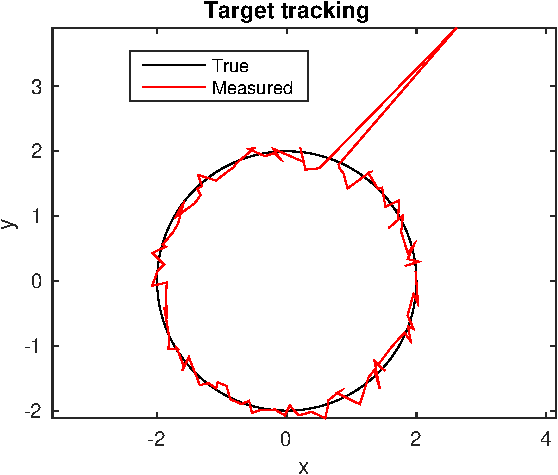
\includegraphics[width=0.9\linewidth]{circular-movement-crop}
\end{center}
\end{column}
\end{columns}
\end{frame}
\begin{frame}[label=sec-1-4]{Example 1 contd.}
The model of the dynamics: \emph{Nearly constant velocity model}
\begin{equation*}
x(k+1) = \bbm I & hI\\ 0 & I \ebm x(k) + \bbm \frac{h^2}{2} I\\hI\ebm v(k),
\end{equation*}
where the state vector contains the position and velocity of the target
\[ x = \bbm p\\\dot{p} \ebm.\]
\end{frame}
\begin{frame}[label=sec-1-5]{Example 1 contd.}
\begin{columns}
\begin{column}{0.3\textwidth}
Result of tracking using standard Kalman filter
\end{column}
\begin{column}{0.7\textwidth}
\begin{center}
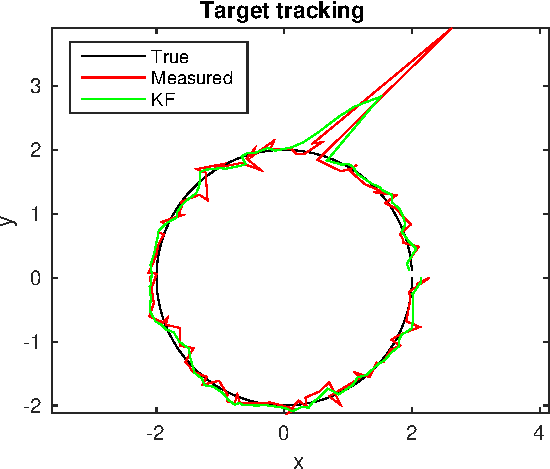
\includegraphics[width=0.9\linewidth]{circular-movement-kf-crop}
\end{center}
\end{column}
\end{columns}
\end{frame}
\section{Convex optimization}
\label{sec-2}
\begin{frame}[label=sec-2-1]{Recommended reading}
\begin{center}
\includegraphics[width=0.8\linewidth]{real-time-convex-opt}
\end{center}
Mattingley, Jacob, and Stephen Boyd. "Real-time convex optimization in signal processing." Signal Processing Magazine, IEEE 27.3 (2010): 50-61.
\end{frame}

\begin{frame}[label=sec-2-2]{Preperation exercise}
Linear regression model
\begin{equation*}
y(k) = ax(k) + b + e(k) + w(k), 
\end{equation*}
where $e(k)$ is Gaussian noise and $w(k)$ is a sparse vector of outliers.
\end{frame}

\begin{frame}[label=sec-2-3]{Preparation exercise, contd}
Least squares estimation:
\begin{equation*}
 \text{minimize} \; ||y - ax - b||_2\\
\end{equation*}
Or, equivalently
\begin{align*}
 \text{minimize} \; & ||\epsilon||_2\\
 \text{subject to} \; & \epsilon = y - ax-b
\end{align*}
\end{frame}


\begin{frame}[label=sec-2-4]{Preparation exercise, contd}
Least squares estimation:
\begin{equation*}
 \text{minimize} \; ||y - ax - b||_2\\
\end{equation*}
Solved by forming 
\[ A = \bbm x(1) & 1\\x(2) & 1\\ \vdots & \vdots\\ x(N) & 1\ebm \]
and
\[ z = \bbm a\\b\ebm, \]
and solving for $z$ in the (over-determined) system of equations
\[ Az = y. \]
\end{frame}
\begin{frame}[label=sec-2-5]{The problem with least squares}
\begin{columns}
\begin{column}{0.4\textwidth}
\begin{align*}
 \text{minimize} \; &\sum_k \phi_{S}(\epsilon_k)\\
 \text{where} \; \phi_S(u) &= u^2
\end{align*}
\end{column}

\begin{column}{0.6\textwidth}

\begin{center}
  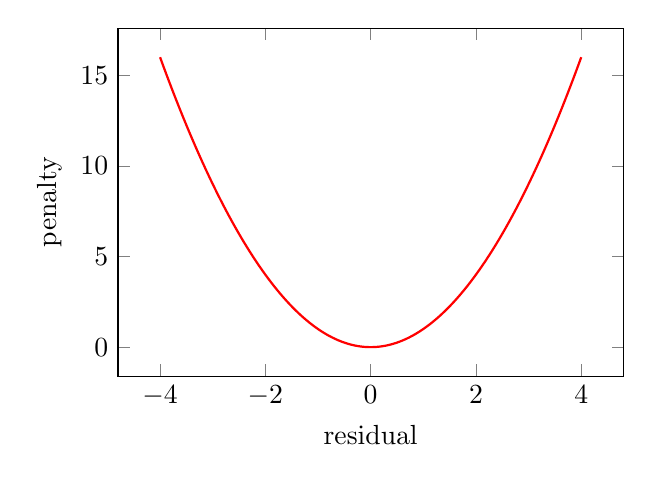
\begin{tikzpicture}
    \begin{axis}[
      width=8cm,
      height=6cm,
      ylabel=penalty,
      xlabel=residual,
      ]
      \addplot[red, thick, no marks, domain=-4:4, samples=201] {x^2};
    \end{axis}
  \end{tikzpicture}
\end{center}
\end{column}
\end{columns}
\end{frame}

\begin{frame}[label=sec-2-6]{More robust: The Huber penalty function}
\begin{columns}
\begin{column}{0.4\textwidth}
A.k.a \emph{robust least squares}
\begin{align*}
 \text{minimize} \; &\sum_k \phi_{hub}(\epsilon_k)\\
 \text{where}\; phi_{hub}(u) &= \begin{cases} u^2 & |u| \le M\\ M(2|u|-M) & |u| > M \end{cases}
\end{align*}
\end{column}

\begin{column}{0.6\textwidth}
\begin{center}
  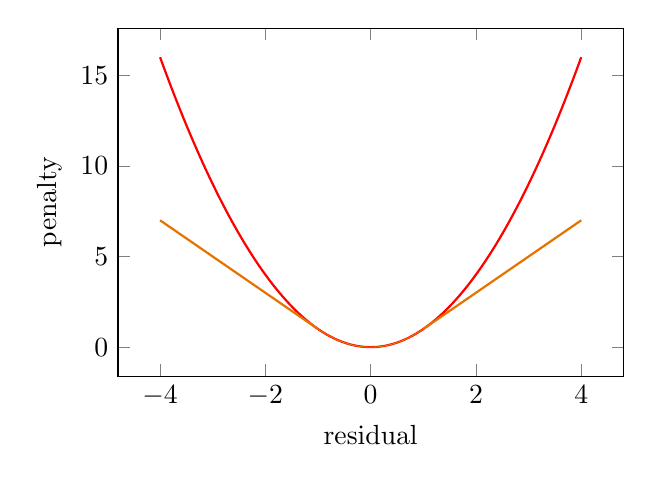
\begin{tikzpicture}
    \begin{axis}[
      width=8cm,
      height=6cm,
      ylabel=penalty,
      xlabel=residual,
      ]
      \addplot[red, thick, no marks, domain=-4:4, samples=201] {x^2};
      \addplot[orange!90!black, thick, no marks, domain=-4:-1, samples=201] {2*abs(x)-1};
      \addplot[orange!90!black, thin, no marks, domain=-1:1, samples=201] {x^2};
      \addplot[orange!90!black, thick, no marks, domain=1:4, samples=201] {2*abs(x)-1};
    \end{axis}
  \end{tikzpicture}
\end{center}
\end{column}
\end{columns}
\end{frame}

\begin{frame}[label=sec-2-7]{Preparation exercis contd.}
l1-regularization:
\begin{equation*}
 \text{minimize} \; ||y - ax - b - w||_2 + \gamma ||w||_1\\
\end{equation*}
Solved by convex optimization.

The vector $w$ will contain the outliers. The larger the value of $\gamma$, the fewer non-zero elements in $w$. 
\end{frame}

\section{Robust Kalman Filter}
\label{sec-3}
\begin{frame}[label=sec-3-1]{The update step of the Kalman filter}
We have the state space model
\begin{align*}
x(k+1) &= Hx(k) + Fv(k)\\
y(k) &= Cx(k) + w(k) + z(k)
\end{align*}
where
\begin{align*}
w &\sim \mathcal{N}(0,R)\\
v &\sim \mathcal{N}(0,Q)
\end{align*}
The measurement update of the Kalman filter can be shown to be equivalent to solving the problem
\[ \text{minimize} \; w^{\mathrm{T}} R^{-1} w + (x-\hat{x}_{k|k-1})P^{-1}(x-\hat{x}_{k|k-1}) \]
\[ \text{subject to}\quad y = Cx + w \]
with variables $w$ and $x$.
\end{frame}
\begin{frame}[label=sec-3-2]{Robust update}
The idea is to write the update step using l1-regularization:
\[ \text{minimize} \; w^{\mathrm{T}} R^{-1} w + (x-\hat{x}_{k|k-1})P^{-1}(x-\hat{x}_{k|k-1}) + \lambda||z||_1 \]
\[ \text{subject to}\quad y = Cx + w + z \]
with variables $w$, $x$ and $z$. The matrix $P$ is the covariance of the prediction error
\[ P = P_{k|k-1} = \mathrm{E} (x-\hat{x}_{k|k-1})(x-\hat{x}_{k|k-1})^{\mathrm{T}}. \]
The parameter $\lambda$ is tuned so that $z$ has desired sparsity.
\end{frame}
\begin{frame}[label=sec-3-3]{Robust update alternative form}
The minization problem of the previous slide can be shown (next slide) to be equivalent to the problem
\[ \text{minimize} \; (e-z)^{\mathrm{T}} S (e-z) + \lambda||z||_1 \]
with variable $z$. To compute $S$, first compute the Kalman gain
\[ K = PC^{\mathrm{T}}(CPC^{\mathrm{T}} + R)^{-1}, \]
and then
\[ S = (I-CK)^{\mathrm{T}} R^{-1} (I-CK) + K^{\mathrm{T}} P^{-1} K. \]

The update is finally computed as
\[ x = \hat{x}_{k|k-1} + K(e-z) \]
\end{frame}
\begin{frame}[label=sec-3-4]{Obtaining the alternative form}
Start with the criterion 
\[ \text{minimize} \; w^{\mathrm{T}} R^{-1} w + (x-\hat{x}_{k|k-1})P^{-1}(x-\hat{x}_{k|k-1}) + \lambda||z||_1. \]
Substitute    \[ x = \hat{x}_{k|k-1} + K(e-z), \]
\[ w = y - Cx - z\] 
and use the identity \[e = y-C\hat{x}_{k|k-1}.\] The alternative form follows.
\end{frame}

\begin{frame}[label=sec-3-5]{Tracking example again}
\begin{columns}
\begin{column}{0.7\textwidth}
\begin{center}
   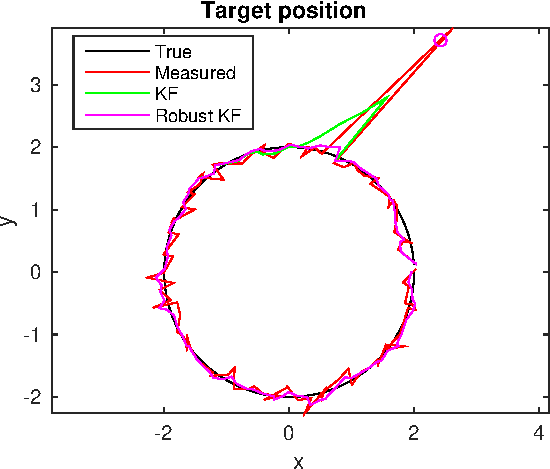
\includegraphics[width=0.9\linewidth]{circular-movement-rkf-crop}
   \end{center}
\end{column}
\end{columns}
\end{frame}

\begin{frame}[label=sec-3-6]{Tracking example again}
\begin{columns}
\begin{column}{0.3\textwidth}
10\% chance of outlier with 10 times normal standard deviation
\end{column}

\begin{column}{0.7\textwidth}
\begin{center}
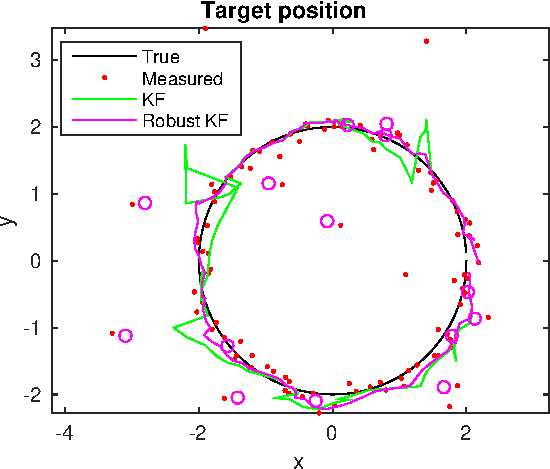
\includegraphics[width=0.9\linewidth]{circular-movement-rkf-2-crop}
\end{center}
\end{column}
\end{columns}
\end{frame}

\begin{frame}[label=sec-3-7]{A fast and approximate implementation}
The optimization problem is
\[ \text{minimize} \; 0.5(e-z)^{\mathrm{T}} S (e-z) + \lambda||z||_1. \]
If $S$ is diagonal, then we can assume the elements of $e$ and $z$ to have the same sign.
The criterion can then be written
\[ \text{minimize} \; 0.5(e-z)^{\mathrm{T}} S (e-z) + \lambda \sign(e)^{\mathrm{T}}z. \]
Expanding the quadratic form leads to
\[\text{minimize} \; 0.5e\transp Se - e\transp S z + 0.5z\transp S z + D\transp z\]
\[ \Rightarrow \; \text{minimize} \;  0.5z\transp S z + C\transp z = f \] 
Which has the solution obtained by setting the derivative of $f$ wrt to $z$ to zero: 
\[df/dz = Sz + C = 0 \]
hence
\[ z = -S^{-1}C = e - \lambda S^{-1}\sign(e). \]
\end{frame}

\begin{frame}[label=sec-3-8]{A fast and approximate implementation, contd}
\begin{block}{Note that we had assumed that the corresponding elements of $z$ and $e$ had the same sign. So, we need to check that this is the case and set to zero those elements of $z$ that do not fulfill this requirement.}
\end{block}
\begin{block}{The method is only guaranteed to work for diagonal \(S\). If \(S\) is not diagonal, an approximate solution can be found by forcing it to be diagonal. The inverse is then trivial to compute.}
\end{block}
\end{frame}

\begin{frame}[fragile,label=sec-3-9]{A fast and approximate implementation, contd}
 Matlab code
\begin{verbatim}
% Compute weighting matrix
% Have Kalman gain K, pred covariance Pkk
% and innovations ek = y - xk1
ICK = eye(m)-C*K;
S = ICK' / R * ICK + K' / Pkk * K;
% Works only if S is diagonal, so lets force it
% We will need the inverse only
Sinv = diag(1.0./diag(S));
se = sign(ek);
z = ek - lambda*Sinv*se;
z(find(sign(z) ~= se)) = 0;
% Filter update
xkNew = xk1 + K*(ek - z);
\end{verbatim}
\end{frame}
% Emacs 25.3.50.2 (Org mode 8.2.10)
\end{document}